\chapter{Marco Teórico}
\label{cap:marcoTeorico}

\section{Sistemas de Procesamiento de \textit{Streaming}}

Entre los diferentes motores de procesamiento de datos masivos, existen los motores de \textsl{streaming}, los cuales reciben grandes cantidades de datos que deben procesar de forma distribuida y \textsl{online}. Para realizar esto, se requiere un cambio en el paradigma \textsl{bash processing}, el cual guarda los datos en una base de datos, los cuales luego son procesados de forma \textsl{offline} \cite{HawwashN14}, a uno que procese de forma \textsl{online}. Por lo que el paradigma cambia a uno basado en grafos, donde a través del cual fluye un \textsl{stream} de datos que es procesamiento por el conjunto de operadores que lo componen, los operadores corresponden a los nodos del grafo y las aristas a los flujos de datos preprocesados que salen del operador \citep{Shahrivari14}.

El modelo de procesamiento que se muestra en la Figura \ref{fig:grafo}, corresponde a un SPS (Sistema de Procesamiento de \textit{Streaming}). Los vértices corresponden a operadores, como por ejemplo analizadores de sentimientos, filtros de palabras o algún algoritmo en particular, y las aristas corresponden a los flujos de datos entre un operador y otro. Además de esto, se tiene una fuente de datos, la cual entrega los datos iniciales a los primeros operadores del grafo \citep{AppelFFB12}.

\begin{figure}[ht!]
  \centering
    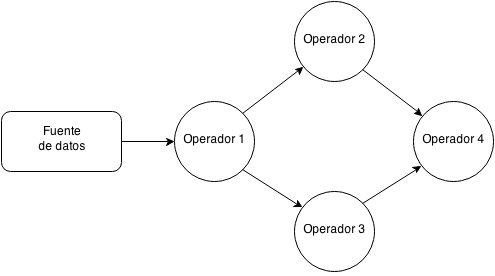
\includegraphics[scale=0.5]{images/Grafo.png}
  \caption{Ejemplo de modelo de SPE.}
  \label{fig:grafo}
\end{figure}

Cada motor de procesamiento de \textsl{streaming} está basado en un modelo de procesamiento en particular. Por ejemplo, S4 está basado en el modelo de procesamiento \textsl{push} \citep{s4yahoo}, y Storm en el modelo \textsl{pull} \citep{stormtwitter}. El primer modelo consiste en el envío de datos desde el operador. La ventaja de este modelo empleado por S4 radica en la abstracción en el envío de datos, sin embargo no asegura el procesamiento de estos, debido a que no existe un mensaje de respuesta al ser entregado al operador. En cambio, en el segundo modelo se basa en la petición de datos a un operador, por lo que son enviados solo si son requeridos. Si bien este modelo asegura procesamiento de los datos, genera una menor abstracción al programador, dado que en el primer modelo sólo se programa a que operador debe ir, en cambio en el segundo se debe indicar quién lo envía y quién lo recibe.

Pues bien, independiente del método que se utilice, existe un problema en la distribución, dado el dinamismo de los datos a procesar, pudiendo generarse sobrecargas en algún operador. Esto se produce dado que la tasa de procesamiento es menor a la tasa de llegada, generando colas en el sistema \citep{queueingtheory}. Por ejemplo, si se posee una tasa de llegada $\lambda$ y una tasa de servicio $\mu$, donde $\mu < \lambda$, se generan colas en el sistema, debido que se procesa más lento de lo que llegan los datos. Como existen colas, es necesario un aumento del rendimiento del sistema, debido que $\rho > 1 $, donde se define $\rho = \frac{\lambda}{s\mu}$, siendo $s$ la cantidad de servicios disponibles.

\section{Balance de carga}

Dentro de la literatura se han encontrado distintas perspectivas al problema de balance de carga en un SPS (Sistema de Procesamiento de \textsl{Streaming}), las cuales consideran los recursos físicos o lógicos como problemas de la sobrecarga del sistema.

\subsection{Recursos físicos}
En esta perspectiva se toma en consideración la sobrecarga del sistema dado las limitantes físicas que éste posea, ya sea por condiciones de los recursos disponibles o por el ambiente de desarrollo. Para esto, se consideran distintos parámetros como umbrales, los cuales si son sobrepasados debe aplicarse alguna estrategia para aliviar la carga del sistema. Estos umbrales pueden ser el nivel SLO, porcentaje de CPU utilizada o disponibilidad de la memoria.

Una de las soluciones con la perspectiva anterior es el Borealis \citep{XingZH05}, donde considerará la cantidad de carga de los nodos en ventanas de tiempo determinadas, las cuales serán manejadas por un coordinador centralizado. Por lo que este coordinador estará encargada de analizar los recursos del sistema, y en caso de sobrepase el umbral propuesto, se deberán emigrar los operadores que estén en ese nodo, para luego ser enviados a otro nodo candidato con menor cantidad de carga. Para elegir al nodo candidato, se realizó una análisis de la cantidad de correlación que existe entre el operador y el nodo candidato, de esta manera, no necesariamente iba a ser enviado a otro nodo con menor sobrecarga, sino también a uno que posea menor cantidad de mensajes. Dentro de los problemas que pueden existir en el sistema es la conexión entre los distintos nodos, por lo que para las pruebas se consideró un buen ancho de banda, de tal manera que aparente una red sin limitaciones de recursos.

\subsection{Recursos lógicos}
%A diferencia de la física, aquí se consideran los componentes lógicos del sistema, como por ejemplo, una sobrecarga en algún operador. De esta manera, en las distintas soluciones se pueden encontrar soluciones en cuanto a la carga existente en el operador o la cantidad de cola que posea, de tal manera, que estos sean los umbrales a considerar para generar una mejora en el sistema.

A diferencia de la física, en esta perspectiva se consideran los componentes lógicos del sistema, como la carga de un operador. Por lo que las distintas soluciones que se presentan, analizan la componentes como el flujo de datos o el tamaño de la cola de un operador, tomando esos parámetros como umbrales en los algoritmos implementados para realizar mejoras en el sistema.

% Enfoques de la perspectiva lógica

Dado esta perspectiva, se han presentando dos tipos de enfoques: el estático y el dinámico \citep{Dong06schedulingalgorithms}. El primer enfoque está centrado en un modelo definido y fijo antes de la inicialización del sistema, sin considerar el estado del sistema. En cambio, el segundo enfoque está basado en un modelo que analizará el sistema según su estado en el transcurso de su ejecución.

%El primer enfoque se centra en la confección de un modelo definido y fijo antes de iniciar el sistema y que no varía en el tiempo. En cambio, el segundo se basa en la adaptación del sistema según su estado en tiempo de ejecución.

\subsection{Enfoque estático}

Este enfoque se ha implementando en distintos motores de \textsl{streaming}, donde no se depende del estado del sistema \citep{stormtwitter, s4}. De esta manera, no existe una interrupción en la ejecución o un cambio en las variables \citep{CasavantK88}. Esto significa, que al momento de distribuir los distintos operadores, esto se realiza homogéneamente, independiente de la carga, latencia u otro estado del sistema.

\textsl{Storm} utiliza la técnica de distribución de operadores según alguna política, tomando el enfoque estático \citep{stormtwitter}. El sistema configura el número de operadores que son necesarios para realizar una tarea, para que después estos sean repartidos en los distintos nodos disponibles según la política de \textit{Shuffle grouping}. Esta técnica basada en algoritmos de planificación \citep{bookScheduling}, consiste en distribuir los operadores en los distintos nodos utilizando una planificación \textsl{Round-Robin}, de tal manera que la cantidad de operadores sea uniforme en los nodos del sistema \citep{bookstorm}.

Otra técnica es el uso de la función \textsl{hash} \citep{RogawayS04} para distribuir los operadores en el grafo, como lo planteado en S4 \citep{s4yahoo}. Esto consiste en aplicar lo anterior a algún atributo del evento, mapeando el evento al operador que corresponda de los $n$ operadores disponibles según el valor de la función. Cabe destacar que si no existe un operador mapeado con la imagen de la función, el sistema clona uno existente evaluando el nuevo con la imagen de la función como identificador. De esta manera, esta técnica provee dinamicidad respecto a la cantidad de operadores en el sistema.

Una ventaja del enfoque estático es el bajo costo de la implementación de los métodos, lo cual es beneficioso para sistemas con bajos recursos. Por otra parte, una desventaja existente es la sobrecarga de un nodo u operador, debido que no asegura que alguno de ellos tenga una mayor tasa de procesamiento que la tasa de llegada. Si bien, no es una solución óptima, es un buen complemento para un modelo con el enfoque dinámico.

\subsection{Enfoque dinámico}

Este enfoque está basado en el estado del sistema, donde según las variables y estado de cada uno de sus atributos, genera una acción en el sistema \citep{CasavantK88}. Esto significa que si el sistema posee alguna anomalía, como una sobrecarga en un operador o latencia entre distintos nodos, se realiza un cambio en el sistema, con el fin de solucionar estos problemas. Para poder dar una solución al problema de sobrecarga, se pueden utilizar dos tipos de modelos: reactivo y predictivo.

\subsubsection{Reactivo}

Este modelo está basado en la detección de sobrecargas en el sistema a través de un monitor \citep{GulisanoJPSV12}. El monitor recibe periódicamente la carga de cada uno de los nodos u operadores, y en caso que se sobrepase un umbral, se aplica una técnica para aumentar el rendimiento bajo una métrica dada. El umbral puede estar basado en el tiempo de procesamiento, el tamaño de la cola u otra variable del nodo u operador \citep{BhuvanagiriGKS06}. Por ejemplo, para realizar una paralelización de un operador sobrecargado, se utiliza un algoritmo que analiza si los operadores sobrepasan un umbral propuesta, el cual está determinado por la frecuencia máxima de llegada de ellos según el tasa de procesamiento del operador \citep{SchneiderAGBW09}.

\subsubsection{Predictivo}
El modelo predictivo está basado en modelos matemáticos que puedan simular la actividad del operador, y predecir la carga de éste. Primero se determina la carga de un operador en cierto período de tiempo, y después se aplica un modelo matemático que predice la carga en el próximo intervalo de tiempo. La predicción de carga de cada operador se realiza mediante modelos de Markov \citep{GongGW10}, y analizando si existe alguna sobrecarga en los operadores a futuro. Si bien lo anterior no ha sido implementando en el contexto de \textsl{Stream}, si se ha realizado en \textsl{Cloud Computing} según la sobrecarga de los computadores \citep{NguyenSGSW13}.\\

Existen distintas técnicas que son utilizadas en ambos modelos, entre las cuales están la planificación determinista \citep{XuCTS14, DongTS07}, descarte de eventos \citep{SheuC09}, migración \citep{XingZH05}, para\-lelización \citep{GulisanoJPSV12, IshiiS11, GedikSHW14} y replicación \citep{FernandezMKP13}.

La planificación determinista \citep{DongTS07} se centra en la planificación según los recursos y estados del sistema \textsl{a priori} según alguna métrica \citep{XuCTS14}. Una métrica utilizada es la frecuencia de datos estimada en un nodo u operador \citep{Ganguly09}. Esta técnica se utiliza, por ejemplo, en \textsl{StreamIt} \citep{ThiesKA02}. Una de las limitaciones es que si bien realiza una predicción determinista de la frecuencia, no necesariamente es correcta a futuro, por lo que no se puede predecir las tasas de tráfico en el transcurso del procesamiento, sino sólo estimarlas al comienzo de la ejecución del sistema.

Otra estrategia está orientada a descartar eventos de un operador sobrecargado, de tal manera de no generar colas en el sistema. Esta estrategia que si bien no está implementada en el sistema por defecto de S4, puede habilitarse \citep{s4}. Otro ejemplo, es la trasmisión de vídeo \textsl{streaming}, donde se descartan los datos que son de baja calidad, para procesar en su mayoría información de alta calidad \citep{SheuC09}. Esta solución está pensada para disminuir la carga, perdiendo la exactitud de la información debido a la pérdida de datos. Por lo tanto existe una menor fiabilidad en el sistema en caso de realizar operaciones de transacción \citep{bookDistrSys}.

También se encuentra la migración, en el cual según el estado del sistema se migran los operadores de un nodo a otro. En \citep{XingZH05} se implementa   esta técnica, y si bien genera una menor carga en distintos nodos, produce un alto costo en la transferencia de los datos. Al realizar la transferencia de los datos, existe una menor tolerancia a fallos, a raíz de lo cual, se propone el uso de un búffer en el sistema, aumentando sus costos \citep{PittauACA07}.

Desde otra perspectiva, existen las técnicas de paralelización y replicación, las cuales se utilizan en caso de sobrepasar un umbral, el cual depende de la carga de un operador, nodo, entre otras variables. El primero consiste en paralelizar una tarea, la cual está determinada por un conjunto de operadores, en otro nodo físico \citep{IshiiS11}. En cambio, la replicación consiste en replicar un operador a nivel lógico del grafo \citep{MadsenTZ14}. Una de las características que existen en este tipo de soluciones es la elasticidad, que consiste en la capacidad de aumentar o disminuir la cantidad de operadores según la necesidad del sistema.

Una aplicación de la técnica de paralelización según el enfoque estático, es la paralelización de tareas de Storm \citep{stormtwitterdoc}, donde un conjunto de operadores realizan una tarea, indicado la cantidad de tareas que se desean ejecutar paralelamente en el sistema. Un ejemplo aplicado de esta técnica según el enfoque dińamico es StreamCloud \citep{GulisanoJPSV12}, que dada la cantidad de consultas que van llegando al sistema, se paralelizan las tareas existentes. Uno de los problemas que surge en estos casos son las operaciones con estado, como lo son los contadores o algoritmos de orden. La solución planteada es poseer un operador que realiza la tarea de \textsl{merge}, que consiste en recibir las salidas de las tareas paralelas, agrupando los datos y proporcionando una salida según lo realizado por cada uno de las operaciones \citep{GedikSHW14}.

Por otra parte, se usa la técnica de replicación en una aplicación diseñada por Fernández \citep{FernandezMKP13}. Ésta está enfocada en la replicación de operadores, la cual se activa si se detecta un cuello botella en el procesamiento de los datos. Para la detección, existe un monitor que está recibiendo la carga de cada uno de los procesos, y si es sobrepasado el umbral, debe realizar una petición de replicación al operador sobrecargado.